\documentclass{article}
\usepackage{graphicx}
\usepackage{geometry}
\usepackage{amsmath,mathpazo}
\usepackage{amssymb}
\usepackage{mathtools}
\usepackage{commath}
\usepackage{enumitem}
\usepackage{listings}

\geometry{
  top=20mm,
}
\newcommand{\boldvec}[1]{\boldsymbol{\vec{\textbf{#1}}}}
\newcommand{\capvec}[1]{\boldsymbol{\hat{\textbf{#1}}}}
\newcommand{\bld}[1]{\textbf{#1}}
\newcommand{\ital}[1]{\textit{#1}}
\begin{document}

\title{Introduction to Parallel \&
Distributed Programming\\COL380 - Assignment 1}
\author{Ankesh Gupta\\2015CS10435}

\date{}
\maketitle

\section*{Question 1}

\bld{Common Assumptions:}
\begin{enumerate}
\item Processor is able to fetch two words from memory in single fetch.
\item All stages mentioned in question are part of processor, one after the other.
\item Loop variables are cached and comparison-adder for loop iterations is being maintained using separate hardware, taking negligible time.
\end{enumerate}  

In an unpipelined setting, things are simpler. Each for-loop manipulation of z goes completely through the processor. The clock is unpipelined setting is 1 common clock, with 1 clock cycle period=$(2+1+1+1+1+1+2)ns=9 ns$. The loop executes 1000 times and thus, 
\begin{align*}
\Aboxed{T_{unpipelined} &=(1000*9)ns=9000ns}
\end{align*}

\bld{Extra Assumptions:}
\begin{enumerate}
  \item There are 7 stages in pipeline. They are in order as mentioned in question.
  \item All stages of pipeline share the same clock. The clock period is dictated by the slowest step, which is $2ns$.
  \item Above assumption also ensures no stalls in our execution pipeline.
  \item 2-way Pipelined Processor is interpreted as 2 execution pipelines available parallely.
\end{enumerate}

In pipelined setting, $clock cycle=2ns$, but each instruction travels 7 stages, making in a way, $14ns$ per instruction. But because pipeline architechture exploits \bld{\ital{idealism of stages}}, in an amortized setting, we can obtain 1 instruction per cycle. Since each of the $z[i]$ computations are \bld{\ital{independent}} of each other, we can feed 2 instruction for adjacent computations in 2 pipelines available. Hence, in essence, each pipeline executes $500$ such instructions. One of them, for odd i's and the other, for even i's.
\begin{align*}
T_{pipelined} &=(6*2)ns(filling\_pipeline) + (500*2)ns\\
\Aboxed{T_{pipelined} &=(1012)ns}
\end{align*}

\bld{Note:} The assumption of no bubble in extra assumption section may be relaxed. If clock cycle is reduced to$=1ns$, we realise that each fetch and store operation will lead to pipeline stalls. In such a scenario, pipeline filling takes$=7ns$ and after, each instruction execution is completed in $2ns$. Hence, total time in this case:
\begin{align*}
T_{modified\_pipelined} &=(5*1+2)ns(filling\_pipeline) + (500*2)ns\\
\Aboxed{T_{modified\_pipelined} &=(1007)ns}
\end{align*}

The pipeline stages are shown for first calculations, which had no stalls.

\hspace*{-2.4cm}
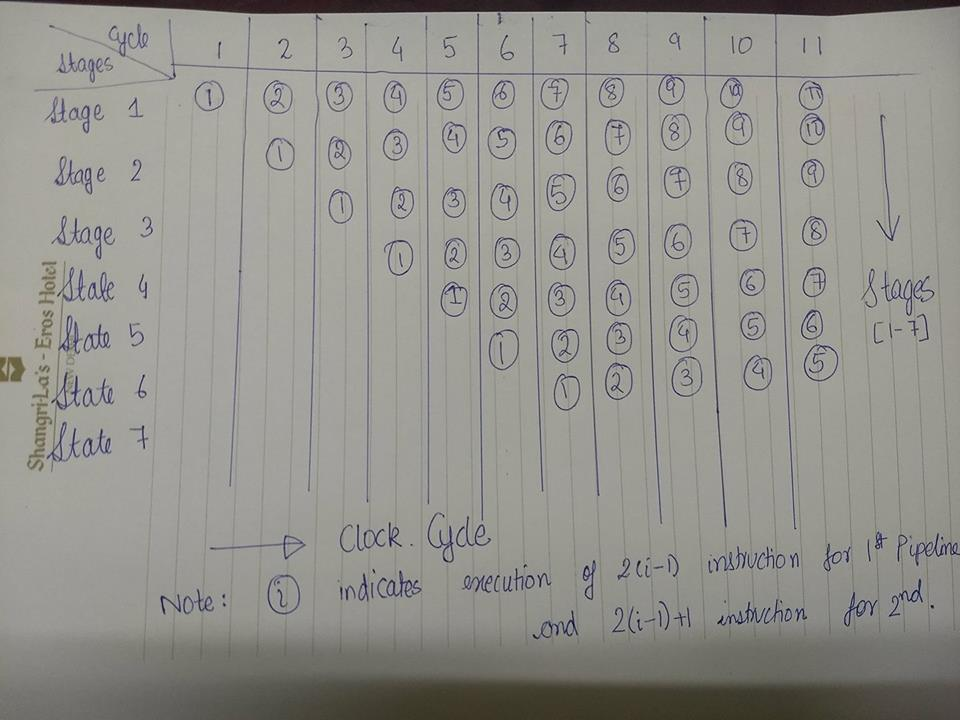
\includegraphics[scale=0.55]{Pipeline.jpg}


\section*{Question 2}
\bld{Assumptions:}
\begin{enumerate}
  \item Since not clear from question, it is assumed that array is $integer array(size 1 word)$ of size $4000 X 4000$.
  \item Prefetching's are ignored to keep calculations simpler.
  \item Data fetched from DRAM is first loaded in cache, and then fetched from cache in subsequent cycles.
  \item Pipeline type fetching from DRAM is ignored.
  \item Again, for loop timings are ignored considering separate hardware taking negligible time.
\end{enumerate}

The problem will be simpler to deal with if we analyze each of the array's independently.\\\\
For $z$ array, a memory access need to be made $once$ every $4$ times loop j executes. Rest 3 times, cache comes in handy.\\
For $x$ array, a memory access need to be made $once$ every $4$ times loop k executes. Rest 3 times fetch is made from cache.\\
For $y$ array, a memory access need to be made $once$ for every iteration of loop k. Since the access's are column major wise, no cache locality could be exploited.\\

Clearly, if we look at k array, then in every 4 iterations of the loop, memory access is made $(4+1)=5$ times for $y(4\_times)$ array and $x(once)$ array respectively. Cache access is done $(4+4+4)=12$ times, 4 times for x,y and z respectively. Hence, for doing $4*2=8$ floating point operations(FLOP), $512 ns$ are required. Hence, in essence, we perform:

\begin{align*}
Performance &=(\frac{8}{512})GFLOPS\\
            &=(0.0156)GFLOPS\\
            &=(15.6)MFLOPS
\end{align*}

\bld{Note:} z DRAM access are kept out of calculation as DRAM access are made once in every ((4*SIZE)*2) floating point operations, to which it has negligible contribution

\section*{Question 3}
Option \bld{2} is correct. The following sequence of events will lead to a \bld{deadlock} situation between the threads. Execute and Loops at below are used with respect to Statement No. mentioned in the question.

\begin{enumerate}

  \item Thread 1 executes 1,2,3,4,5. Loops at 5. $process\_arrived=1$
  \item Thread 2 executes 1,2,3,4,5. Loops at 5. $process\_arrived=2$
  \item Thread 3 executes 1,2,3,4,5 ($process\_arrived=3$,breaks),6,7,8,12,1 \ital{(successive invocation)},2,3,4,5. Loops at 5. $process\_arrived=4, process\_left=1$
  \item No other thread ever breaks free of the loop as $processed\_arrived$ will never be reset again
\end{enumerate}
  
The sequence of operations above leads to \bld{deadlock}, where no thread is able to make any progress. This situation arise because 2 barrier in invocations are used in immediate succession(noted in point 3)\\

The following code is one of the ways of resolving the issue pointed out above.

\begin{verbatim}
void barrier ( void ) {
  L( S ) ;
  process_arrived++;
  UL( S ) ;
  while ( process_arrived!=3) ;
  L( S ) ;
  process_left++;
  UL( S ) ;
  if(process_left==3){
    process_arrived=0;
    process_left=0;
  }
  while(process_left!=0);
}
\end{verbatim}

The above code ensures that all the 3 threads executing the barrier leaves the barrier simultaneously. The flaw in previous snippet was that it synchronised threads momentuously, but their exiting the barrier was independent. Now, the barrier will ensure that all variables have been reset, and even the last thread in opertion pipeline is ready to depart.

% \pagebreak

\section*{Question 4}

Option \bld(b) is correct.\\

\begin{minipage}{0.5\textwidth}
 \begin{lstlisting}
  ****Thread i****
while (true) {
1. flag[i]=true;
2. turn=j;
3. while(flag[j]==true && turn==j);
   /∗ enter critical section
   perform actions
   exit */
4. flag[i]=false ;
   } 
\end{lstlisting}
\end{minipage}
\begin{minipage}{0.5\textwidth}
 \begin{lstlisting}
  ****Thread j****
while (true) {
flag[j]=true;
turn=i;
while(flag[i]==true && turn==i);
/∗ enter critical section
perform actions
exit */
flag[j]=false ;
} 
\end{lstlisting}\end{minipage}


\bld{Justification of Exclusion:} Suppost for sake of contradiction, we assume that both the threads execute critical section simultaneously. WLOG, we assume that thread i executed statement 2 first. So, for thread j to execute critical section, flag[i] must have been false in while loop \bld{(..a)}. If we construct a \bld{happen-before} graph, we realise that Thread i statement 2 must happen before Thread j statement 2(assumption), which must happen before Thread j statement 3(sequentiality), which must happen before Thread i statement 1\bld{(from (..a))}. 

Hence there is a \ital{happen-before loop, which leads to contradiction}. Notice here we assumed the an order of execution of Statement 2 WLOG, hence this completes the proof.\\

\bld{Justification of Liveliness:} Its clear that if only 1 thread is invoking the function, the other threads flag remains false, and thread works uninterrupted. Interesting is when both threads want to access the critical section. Again, the while loop construct ensures that none of the threads executes the critical section in succession, keeping the other thread waiting. Each resetting of \ital{turn} variable is an opportunity for the waiting thread to complete its request of critical section.



\section*{Question 5}
\begin{enumerate}[label=(\alph*)]

\item Lets start by writing the efficiency equation for given system, and doing algebraic manipulations.

\begin{align*}
E &=\frac{T_{serial}}{p*T_{parallel}}
\end{align*}
Substituting from the question, $T_{parallel}$, we get:
\begin{align*}
E &=\frac{T_{serial}}{T_{serial}+p*T_{overhead}}\\
  &=\frac{1}{1+\frac{p*T_{overhead}}{T_{serial}}}
\end{align*}
We know that $T_{serial}$ is same as $W$(input size), the workload, which gives us:
\begin{align*}
E &=\frac{1}{1+\frac{p*T_{overhead}}{W}}
\end{align*}
Assuming that $T_{overhead}$ is a \bld{sublinear} function of Workload$(W)$, the growth in workload dominates the growth in overhead, which decreases the denominator, in turn increasing efficiency. Asymtotically we can write:
\begin{align*}
E &=\frac{1}{1+\frac{p*T_{overhead}}{W}} \approx{1}
\end{align*}

Hence, as input size grows, $Efficiency$ increases, and aymtotically reaches 1. The main assumption is that: $$W = \Omega({T_{overhead}})$$

\item \bld{Scalability} is defined as the ability of parallel system to keep efficiency, when processing units and workload of the system changes.

Lets analyze the given parallel construct and derive iso-efficiency function.

\begin{align*}
E &=\frac{T_{serial}}{p*T_{parallel}}\\
  &=\frac{n}{n+p*\log_2 p}
\end{align*}
Moving terms, and writing $n$ as function of $p(processing units)$, we get:  
\begin{align*}
n &=\frac{E}{1-E}*p\log_2 p\\
\end{align*}
Let initial processing units be $p_1$, and later it changed to $p_2=k*p_1$, corresponding $n_1,n_2$ are:
\begin{align*}
n_1 &=\frac{E}{1-E}*p_1\log_2 p_1\\
n_2 &=\frac{E}{1-E}*k*p_1\log_2 (k*p_1)\\
\Aboxed{\frac{n_2}{n_1} &= k*(1+\frac{log_2 k}{log_2 p_1})}
\end{align*}

Although the system is scalable(because it are able to maintain \ital{isoefficiency}), it is \bld{weakly scalable}. This is because increase in $workload($n$)$ required to attain iso-efficiency is $super-linear$ with respect to processing units, as visible from the last equation. Hence the system is \bld{\ital{weakly scalable}}.

\item The cost optimal version of parallel-sum algorithm for $n$ numbers on $p$ processing units does the following:

\begin{enumerate}[label=(\roman*)]
\item Divide the numbers $equally$ and $exclusively$ amongst the p cores. Each core get $\frac{n}{p}$ numbers.
\item Sum all the numbers each core receives and store the sum locally. This takes $O(\frac{n}{p})$ time.
\item Merge the local sums from each of the cores into a global sum in \ital{divide and conquer} style. This takes $O(log_2 p)$ time.
\end{enumerate}  

Examining the above algorithm, running time of above algorithm is $T_{parallel}=O(\frac{n}{p} + \log_2 p)$. The best serial algorithm sums up the numbers in $T_{serial}=O(n)$ time. Analyzing the cost: 
\begin{align*}
C_{s} &=T_{serial}=n\\
C_{p} &=p*T_{parallel}=n+p*\log_2 p\\
\frac{C_{p}}{C_{s}} &=1+\frac{p*\log_2 p}{n}
\end{align*}

As long as $n=\Omega(p*\log_2 p)$, the above parallel construct is cost optimal, as then asymtotically:
\begin{align*}
\Aboxed{C_p &=\Theta(C_s)}
\end{align*}
\end{enumerate}

Deriving expressions for terms asked in question, $T_{parallel}$ has already been written above in runtime analysis. Substituting the values for summing,

\begin{align*}
T_{parallel} &=\frac{n}{p} + \log_2 p\\
  &= \frac{n}{p}*1 + \log_2 p*(20+1)(Substituting)\\
\Aboxed{T_{parallel} &= \frac{n}{p} + \log_2 p*(21)}
\end{align*}

For \bld{speedup($S$)},
\begin{align*}
S &=\frac{T_{serial}}{T_{parallel}}\\
  &= \frac{n}{\frac{n}{p}+log_2 p}\\
\Aboxed{S &= \frac{p}{1+\frac{p*log_2 p*21}{n}}} (Substituting)
\end{align*}
For \bld{efficiency($E$)},
\begin{align*}
E &= \frac{T_{serial}}{p*T_{parallel}}\\
  &= \frac{n}{p*(\frac{n}{p}+log_2 p)}\\
  &= \frac{n}{n+p*\log_2 p}\\
  &= \frac{n}{n+p*\log_2 p*21}(Substituting)\\
\Aboxed{E &= \frac{1}{1+\frac{p*\log_2 p*21}{n}}}
\end{align*}

Equations for \bld{Cost} had been derived while prooving optimality. What remains is substitution of time.
\begin{align*}
C_{s} &=T_{serial}=n\\
C_{p} &=p*T_{parallel}=n+p*\log_2 p*21\\
\Aboxed{\frac{C_{p}}{C_{s}} &=1+\frac{p*\log_2 p*21}{n}}
\end{align*}

\bld{Iso-efficiency} can be derived from Efficiency equation, by algebraic manipulations.
\begin{align*}
E &= \frac{n}{p*(\frac{n}{p}+log_2 p*21)}\\
n*(1-E) &= E*p*log_2 p*21\\
\Aboxed{n &= \frac{E}{1-E}*p*log_2 p*21}\\
\end{align*}


% \begin{align*}
% u &= u_0 + xu_x + yu_y\\
% v &= v_0 + xv_x + yv_y
% \end{align*}
% The Optical flow equation is:
% $$ uI_x + vI_y + I_t = 0 $$
% Putting the given equation in optical flow equation, we get:
% $$ I_x(u_0 + xu_x + yu_y) + I_y(v_0 + xv_x + yv_y) = -I_t $$
% Now, we take a region around the point $(x,y)$ and we assume that optical flow assumptions
% hold in this region.\\
% Thus, using the above equation, we can transform our case into a least square problem as follows:\\
% Define matrix $\mathbf{A}$ as:
% $$
% \mathbf{A} = \begin{bmatrix}
%   I_x(p1) & x_{p1}I_x(p1) & y_{p1}I_x(p1) & I_y(p1) & x_{p1}I_y(p1) & y_{p1}I_y(p1)\\
%   I_x(p2) & x_{p2}I_x(p2) & y_{p2}I_x(p2) & I_y(p2) & x_{p2}I_y(p2) & y_{p2}I_y(p2)\\
%   \vdots & \vdots & \vdots & \vdots & \vdots & \vdots \\
%   I_x(pn) & x_{pn}I_x(pn) & y_{pn}I_x(pn) & I_y(pn) & x_{pn}I_y(pn) & y_{pn}I_y(pn)
% \end{bmatrix}
% $$
% and $\vec{u}$ and $\vec{b}$ as:
% $$
% \vec{u} = \begin{bmatrix}
%   u_0 \\
%   u_x \\
%   u_y \\
%   v_0 \\
%   v_x \\
%   v_y
% \end{bmatrix}
% \qquad
% \vec{b} = -\begin{bmatrix}
%   I_t(p1) \\
%   I_t(p2) \\
%   \vdots \\
%   I_t(pn)
% \end{bmatrix}
% $$
% and our least square problem becomes
% $$ \min \quad \lVert \mathbf{A}\vec{u} - \vec{b} \rVert^2 $$
% whose solution comes out to be:
% $$ \vec{u} = (A^TA)^{-1}A^Tb$$
% The assumption that we made in this case are:
% \begin{enumerate}
% \item
% The values of the parameter don't change for the $n$ points near $(x,y)$.
% \item
% Matrix $A^TA$ is invertible.
% \end{enumerate}
% \pagebreak

% \section*{Question 6}
% The velocity of the object is:
% $$ V = -U-\Omega \times P $$
% which, when expanded, translates to:
% \begin{align*}
% V_1 &= \frac{dX}{dt} = -U_1 - \Omega_2Z + \Omega_3Y \\
% V_2 &= \frac{dY}{dt} = -U_2 - \Omega_3Z + \Omega_1Z \\
% V_3 &= \frac{dZ}{dt} = -U_3 - \Omega_1Y + \Omega_2X 
% \end{align*}
% Also, it is given that:
% $$
% x=\frac{fX}{Z} \quad y = \frac{fY}{Z}
% $$
% and by vector calculus:
% $$
% u = \frac{dx}{dt} \qquad v = \frac{dy}{dt}
% $$
% and by putting value of $x$ from above:
% \begin{align*}
%   u &= \frac{d(\frac{fX}{Z})}{dt} \\
%     &= f\frac{Z\frac{dX}{dt} - X\frac{dZ}{dt}}{Z^2} \\
%     &= f\frac{ZV_1 - XV_3}{Z^2} \\
%     &= \frac{f}{Z}(-U_1 - \Omega_2Z + \Omega_3Y) - \frac{x}{Z}(-U_3 - \Omega_1Y + \Omega_2X)\\
%     &= -U_1\frac{f}{Z} - \Omega_2f + \Omega_3y - x (-\frac{U_3}{Z} - \frac{\Omega_1y}{f}+\frac{\Omega_2x}{f})
% \end{align*}
% Therefore,\\
% $$u = -U_1\frac{f}{Z} - \Omega_2f + \Omega_3y - x (-\frac{U_3}{Z} - \frac{\Omega_1y}{f}+\frac{\Omega_2x}{f})$$
% Similary, putting value of $y$, we get:
% \begin{align*}
%   v &= \frac{d(\frac{fY}{Z})}{dt} \\
%     &= f\frac{Z\frac{dY}{dt} - Y\frac{dZ}{dt}}{Z^2} \\
%     &= f\frac{ZV_2 - YV_3}{Z^2} \\
%     &= \frac{f}{Z}(-U_2 - \Omega_3Z + \Omega_1Z) - \frac{y}{Z}(-U_3 - \Omega_1Y + \Omega_2X)\\
%     &= -U_2\frac{f}{Z} - \Omega_3x + \Omega_1f - y (-\frac{U_3}{Z} - \frac{\Omega_1y}{f}+\frac{\Omega_2x}{f})
% \end{align*}
% Therefore,\\
% $$v = -U_2\frac{f}{Z} - \Omega_3x + \Omega_1f - y (-\frac{U_3}{Z} - \frac{\Omega_1y}{f}+\frac{\Omega_2x}{f})$$
% Hence Proved.

% \pagebreak
% \section*{Question 7}
% From previous question, it is given that:
% \begin{align*}
% u &= -U_1\frac{f}{Z} - \Omega_2f + \Omega_3y - x (-\frac{U_3}{Z} - \frac{\Omega_1y}{f}+\frac{\Omega_2x}{f}) \\
% v &= -U_2\frac{f}{Z} - \Omega_3x + \Omega_1f - y (-\frac{U_3}{Z} - \frac{\Omega_1y}{f}+\frac{\Omega_2x}{f})
% \end{align*}
% Now, since we are taking first order linear approximation of $u$ and $y$:
% \begin{align*}
% u &= -U_1\frac{f}{Z} - \Omega_2f + \Omega_3y + x\frac{U_3}{Z} +O(x^2,xy,y^2) \\
% v &= -U_2\frac{f}{Z} + \Omega_1f - \Omega_3x + y\frac{U_3}{Z} +O(x^2,xy,y^2)
% \end{align*}
% After taking partial derivative of $u$ w.r.t. $x$ we get:
% \begin{align*}
% \frac{\partial{u}}{\partial{x}} &= U_1f\frac{\frac{\partial{Z}}{\partial{x}}}{Z^2}
%                                 + 0 + 0 + \frac{U_3}{Z} - xU_3\frac{\frac{\partial{Z}}{\partial{x}}}{Z^2} \\
%                                 &= U_1f\frac{Z_x}{Z^2} + \frac{U_3}{Z} + \textit{(tending to 0 terms)} \\
% \Aboxed{\therefore u_x &= U_1f\frac{Z_x}{Z^2} + \frac{U_3}{Z}}\\
% \end{align*}
% Similarly, for others:
% \begin{align*}
% \frac{\partial{u}}{\partial{y}} &= U_1f\frac{\frac{\partial{Z}}{\partial{y}}}{Z^2}
%                                 + 0 + \Omega_3 + 0 - xU_3\frac{\frac{\partial{Z}}{\partial{y}}}{Z^2} \\
%                                 &= U_1f\frac{Z_y}{Z^2} + \Omega_3 + \textit{(tending to 0 terms)} \\
% \Aboxed{\therefore u_y &= U_1f\frac{Z_y}{Z^2} + \Omega_3}\\
% \frac{\partial{v}}{\partial{x}} &= U_2f\frac{\frac{\partial{Z}}{\partial{x}}}{Z^2}
%                                 + 0 - \Omega_3 + 0 - yU_3\frac{\frac{\partial{Z}}{\partial{x}}}{Z^2} \\
%                                 &= U_2f\frac{Z_x}{Z^2} - \Omega_3 + \textit{(tending to 0 terms)} \\
% \Aboxed{\therefore v_x &= U_2f\frac{Z_x}{Z^2} - \Omega_3}\\
% \frac{\partial{v}}{\partial{y}} &= U_2f\frac{\frac{\partial{Z}}{\partial{y}}}{Z^2}
%                                 + 0 + 0 + \frac{U_3}{Z} - yU_3\frac{\frac{\partial{Z}}{\partial{y}}}{Z^2} \\
%                                 &= U_2f\frac{Z_y}{Z^2} + \frac{U_3}{Z} + \textit{(tending to 0 terms)} \\
% \Aboxed{\therefore v_y &= U_2f\frac{Z_y}{Z^2} + \frac{U_3}{Z} }\\
% \end{align*}

% Given:
% \begin{align*}
%   V_z = \frac{U_3}{Z}, \quad V_x = \frac{U_1}{Z}, \quad V_y = \frac{U_2}{Z},
%   \quad Z_X = \frac{fZ_x}{Z} \quad\textit{and}\quad Z_Y = \frac{fZ_y}{Z}
% \end{align*}
% We get:
% \begin{alignat*}{3}
% u_x \quad &= \quad U_1f\frac{Z_x}{Z^2} + \frac{U_3}{Z} \quad &&= \quad V_z + V_xZ_X\\
% u_y \quad &= \quad U_1f\frac{Z_y}{Z^2} + \Omega_3 \quad &&= \quad \Omega_3 + V_xZ_Y\\
% v_x \quad &= \quad U_2f\frac{Z_x}{Z^2} - \Omega_3 \quad &&= \quad -\Omega_3 + V_yZ_X\\
% v_y \quad &= \quad U_2f\frac{Z_y}{Z^2} + \frac{U_3}{Z} \quad &&= \quad V_z + V_yZ_Y\\
% \end{alignat*}
% Hence Proved.
% \section*{Question 8}
% Given statements:
% \begin{align*}
%   div\mathbf{v} &= (u_x+v_y) \\
%   curl\mathbf{v} &= -(u_y-v_x) \\
%   (def\mathbf{v})cos2\mu &= (u_x - v_y) \\ 
%   (def\mathbf{v})sin2\mu &= (u_y + v_x) \\ 
% \end{align*}
% Putting values in the equation:
% $$
%   \frac{div\mathbf{v}}{2}\begin{bmatrix}1&0\\0&1\end{bmatrix}
% + \frac{curl\mathbf{v}}{2}\begin{bmatrix}0&-1\\1&0\end{bmatrix}
% + \frac{def\mathbf{v}}{2}\begin{bmatrix} cos2\mu & sin2\mu \\ sin2\mu & -cos2\mu \end{bmatrix}
% $$
% we get :
% \begin{align*}
%   &= \frac{(u_x+v_y)}{2}\begin{bmatrix}1&0\\0&1\end{bmatrix}
% + \frac{(v_x - u_y)}{2}\begin{bmatrix}0&-1\\1&0\end{bmatrix}
% + \frac{def\mathbf{v}}{2}\begin{bmatrix} cos2\mu & sin2\mu \\ sin2\mu & -cos2\mu \end{bmatrix}
% \\
%   &= \begin{bmatrix}\frac{(u_x+v_y)}{2}&0\\0&\frac{(u_x+v_y)}{2}\end{bmatrix}
% + \begin{bmatrix}0&\frac{(u_y-v_x)}{2}\\\frac{(v_x - u_y)}{2}&0\end{bmatrix}
% + \begin{bmatrix}(\frac{def\mathbf{v}}{2})cos2\mu &(\frac{def\mathbf{v}}{2})sin2\mu \\
%                   (\frac{def\mathbf{v}}{2})sin2\mu & -(\frac{def\mathbf{v}}{2})cos2\mu \end{bmatrix}
% \\
%   &= \begin{bmatrix} \frac{(u_x+v_y)}{2} &\frac{(u_y-v_x)}{2} \\
%                   \frac{(u_y-v_x)}{2} &\frac{(v_y+u_x)}{2}\end{bmatrix}
% + \begin{bmatrix} \frac{(u_x-v_y)}{2} &\frac{(u_y+v_x)}{2} \\
%                   \frac{(u_y+v_x)}{2} &\frac{(v_y-u_x)}{2}\end{bmatrix}
% \\
%  &= \begin{bmatrix} u_x & u_y \\ v_x & v_y \end{bmatrix}
% \end{align*}
% Therefore,
% $$
% \begin{bmatrix} u_x & u_y \\ v_x & v_y \end{bmatrix}
% = \frac{div\mathbf{v}}{2}\begin{bmatrix}1&0\\0&1\end{bmatrix}
% + \frac{curl\mathbf{v}}{2}\begin{bmatrix}0&-1\\1&0\end{bmatrix}
% + \frac{def\mathbf{v}}{2}\begin{bmatrix} cos2\mu & sin2\mu \\ sin2\mu & -cos2\mu \end{bmatrix}
% $$
% Hence Verified.
% \pagebreak

% \section*{Question 9}
% We know that $\boldsymbol{\hat{\textbf{Q}}}$ is the unit vector in the camera look-at direction. Therefore,
% $$ \boldsymbol{\hat{\textbf{Q}}} = (0,0,1)$$
% Also, $\boldvec{U}$ is the translational velocity of the object. Therefore,
% \begin{align*}
%     \boldvec{U} &= (U_1,U_2,U_3)\\
%     \boldvec{A} &= \frac{\boldvec{U} - (\boldvec{U} \cdot \capvec{Q})\capvec{Q}}{Z} \\
%                 &= \frac{(U_1,U_2,U_3) - (0,0,U_3)}{Z} \\
%     \therefore \boldvec{A} &= \frac{(U_1,U_2,0)}{Z}
% \end{align*}
% Next, we write $\nabla Z$ as:
% \begin{align*}
% \nabla Z &= (\frac{\partial{Z}}{\partial{x}},\frac{\partial{Z}}{\partial{y}},0)
%         = (Z_x,Z_y,0) \\
% \therefore \boldvec{F}&= \frac{f}{Z}\nabla Z = \frac{f}{Z}(Z_x,Z_y,0)
% \end{align*}
% Also, from \textit{Question 8} we have:
% \begin{align*}
%   div\mathbf{v} &= (u_x+v_y) \\
%   curl\mathbf{v} &= -(u_y-v_x) \\
%   (def\mathbf{v})cos2\mu &= (u_x - v_y) \\ 
%   (def\mathbf{v})sin2\mu &= (u_y + v_x) \\ 
% \end{align*}
% And from \textit{Question 7} we have:
% \begin{align*}
% u_x &= U_1f\frac{Z_x}{Z^2} + \frac{U_3}{Z}\\
% u_y &= U_1f\frac{Z_y}{Z^2} + \Omega_3 \\
% v_x &= U_2f\frac{Z_x}{Z^2} - \Omega_3 \\
% v_y &= U_2f\frac{Z_y}{Z^2} + \frac{U_3}{Z}
% \end{align*}
% Putting the values, we get:
% \begin{align*}
%     div\mathbf{v} &= 2\frac{U_3}{Z} + \frac{f}{Z^2}(U_1Z_x + U_2Z_y)\\
%     curl\mathbf{v} &= -2\Omega_3 + \frac{f}{Z^2}(U_2Z_x - U_1Z_y)\\
%     (def\mathbf{v})cos2\mu &= \frac{f}{Z^2}(U_1Z_x - U_2Z_y)\\
%     (def\mathbf{v})sin2\mu &= \frac{f}{Z^2}(U_1Z_y + U_2Z_x)\\ 
% \end{align*}
% Now let us evaluate:
% \begin{align*}
%     & 2\frac{\boldvec{U}\cdot\capvec{Q}}{Z} + \boldvec{F}\cdot\boldvec{A}\\
%     =& 2\frac{(U_1,U_2,U_3)\cdot(0,0,1)}{Z} + \frac{f}{Z}(Z_x,Z_y,0)\cdot \frac{(U_1,U_2,0)}{Z} \\
%     =& 2\frac{U_3}{Z} + \frac{f}{Z^2}(Z_xU_1 + Z_yU_2)\\
%     =& div\mathbf{v}\\
%     \Aboxed{\therefore div\mathbf{v} =& 2\frac{\boldvec{U}\cdot\capvec{Q}}{Z} + \boldvec{F}\cdot\boldvec{A}}\\
% \end{align*}
% Similarly, for others:
%     % -2\boldvec{\Omega} \cdot \capvec{Q} + \abs{ (\boldvec{F} \times \boldvec{A}) }
% \begin{align*}
%     &-2\boldvec{$\Omega$} \cdot \capvec{Q} + \abs{ (\boldvec{F} \times \boldvec{A}) }\\
%     =& -2(\Omega_1,\Omega_2,\Omega_3)\cdot(0,0,1) + \abs{\frac{f}{Z}(Z_x,Z_y,0)\times \frac{(U_1,U_2,0)}{Z}}\\
%     =& -2\Omega_3 + \abs{\frac{f}{Z^2}(0,0,U_2Z_x - U_1Z_y)}\\
%     =& -2\Omega_3 + \frac{f}{Z^2}(U_2Z_x - U_1Z_y)\\
%     =& curl\mathbf{v}\\
%     \Aboxed{\therefore curl\mathbf{v} =& -2\boldvec{$\Omega$} \cdot \capvec{Q} + \abs{ (\boldvec{F} \times \boldvec{A}) }}
% \end{align*}

% Now :
% \begin{align*}
%   def\mathbf{v} &= \sqrt{((def\mathbf{v})cos2\mu)^2 + ((def\mathbf{v})sin2\mu)^2}\\
%                 &= \frac{f}{Z^2}\sqrt{ U_1^2Z_x^2 + U_2^2Z_y^2 + U_2^2Z_x^2 + U_1^2Z_y^2 }\\
%                 &= \frac{f}{Z^2}\sqrt{U_1^2 + U_2^2}\sqrt{Z_x^2 + Z_y^2}\\
%                 &= \abs{\frac{(U_1,U_2,0)}{Z}} + \abs{\frac{f}{Z}(Z_x,Z_y,0)}\\
%                 &= \abs{\boldvec{F}}\abs{\boldvec{A}} \\
%   \Aboxed{\therefore def\mathbf{v} &= \abs{\boldvec{F}}\abs{\boldvec{A}} }
% \end{align*}
% Finally,
% \begin{align*}
% tan2\mu &= \frac{(def\mathbf{v})sin2\mu}{(def\mathbf{v})cos2\mu}\\
%         &= \frac{\frac{f}{Z^2}(U_1Z_y + U_2Z_x)}{\frac{f}{Z^2}(U_1Z_x - U_2Z_y)}\\
%         &= \frac{(U_1Z_y + U_2Z_x)}{(U_1Z_x - U_2Z_y)}\\
%         &= \frac{(\frac{Z_y}{Z_x} + \frac{U_2}{U_1})}{(1 - \frac{U_2}{U_1}\frac{Z_y}{Z_x})}\\
% \end{align*}
% And we already have:
% \begin{align*}
%   tan(\angle A) = \frac{U_2}{U_1} \qquad tan(\angle F) = \frac{Z_y}{Z_x}
% \end{align*}
% Therefore,
% \begin{align*}
%   tan2\mu &= \frac{tan(\angle A)+tan(\angle F)}{1 - tan(\angle A)tan(\angle F)}\\
%           &= \tan(\angle A + \angle F)\\
%   2\mu &= \angle A + \angle F \\
%   \Aboxed{\therefore \mu &= \frac{(\angle A + \angle F)}{2}}
% \end{align*}
% Hence Proved.

% \section*{Question 10}
% \begin{enumerate}[label=(\alph*)]

% \item Deformation can be used to encode the surface orientation as it gives us an idea of how object deforms
% with small change in object position, thus revealing information about the orientation. Similarly, divergence
% is a measure of how objects scale as they move towards camera, and thus high divergence implies that velocity
% is high and thus time of collision will be shorter. Also, these components are unaffected by viewer rotations
% such as panning or tilting of the camera unlike point image velocities, which change considerably.

% \item If $\boldvec{A}=0$ then $div\mathbf{v} = 2\frac{\boldvec{U}\cdot\capvec{Q}}{Z}$. Also,
% $\boldvec{U}\cdot\capvec{Q}$ encodes the velocity of object in direction of camera and $Z$ is distance of
% object. Thus, time of collision is $\frac{Z}{\boldvec{U}\cdot\capvec{Q}}$ which is $\frac{2}{div\mathbf{v}}$.
% Thus, if $\boldvec{A}=0$ then we can determine time of collision.\\
% Also, in general motion, the time of collision is bounded by:
% $$
% \frac{2}{div\mathbf{v} + def\mathbf{v}} \leq \mathbf{t_c} \leq \frac{2}{div\mathbf{v} - def\mathbf{v}}
% $$

% \item It can be seen that shallow objects that are near to camera will produce same affect as deep structures
% which are far away from camera, because in pinhole model the motion registered are actually scaled components of
% actual motion ($x = f\frac{X}{Z}$) and thus a large motion which is far away will approximate to small motion that
% is near (as their ratio will be of same order).

% \item I think that egomotion can be used to gain some knowledge about the surface orientation, assuming that
% the object in question is actually constant. This is because small changes in the direction of camera look-at direction
% can be used to map the surface gradient of the object, and thus can give us an idea of the orientation of surface of the object.

% \end{enumerate}

% \section*{Declaration of Originality}
% I hereby claim that the work presented here is my own and not copied from anywhere. Though, while writing these
% answers I had discussions with Aman Agrawal (2015CS10210) , Ankesh Gupta (2015CS10435) and Saket Dingliwal (2015CS10254).\\
% These discussions were mainly focused on clearing doubts on the meaning of question and clearing diagramatic representation
% of the given situation. Also, I referred to a paper cited in the References for help in understanding the context and
% background of question 6.\\

% \begin{thebibliography}{1}
%   \bibitem{imagediv} 
%   Roberto Cipolla and Andrew Blake.
%   \textit{Image divergence and deformation from closed curves}.\\ 
%   Int. Journal of Robotics Research, 16(1):77-96, 1997.
% \end{thebibliography}

\end{document}
